%%%%%%%%%%%%%%%%%%%%%%%%%%%%%%%%%%%%%%%%%%%%%%%%%%%%%%%%%%%
% --------------------------------------------------------
% Rho
% LaTeX Template
% Version 2.1.1 (01/09/2024)
%
% Authors: 
% Guillermo Jimenez (memo.notess1@gmail.com)
% Eduardo Gracidas (eduardo.gracidas29@gmail.com)
% 
% License:
% Creative Commons CC BY 4.0
% --------------------------------------------------------
%%%%%%%%%%%%%%%%%%%%%%%%%%%%%%%%%%%%%%%%%%%%%%%%%%%%%%%%%%%

\documentclass[9pt,a4paper,twoside]{rho-class/rho}
\usepackage[english]{babel}

%% Spanish babel recomendation
% \usepackage[spanish,es-nodecimaldot,es-noindentfirst]{babel}

\setbool{rho-abstract}{true} % Set false to hide the abstract
\setbool{corres-info}{true} % Set false to hide the corresponding author section

%----------------------------------------------------------
% TITLE
%----------------------------------------------------------

\journalname{COMP6841 SAP}
\title{Simulating End-to-End Encrypted Based on the Signal Protocol}

%----------------------------------------------------------
% AUTHORS AND AFFILIATIONS
%----------------------------------------------------------

\author[1]{Jinghan Wang  z5286124}


\begin{abstract}
    Signal Protocol represents a state-of-the-art approach to end-to-end encrypted messaging, addressing critical security challenges in modern communication systems. This research examines the protocol's cryptographic foundations, security architecture, and practical implementation aspects. We explore the protocol's core mechanisms, including the X3DH key agreement protocol and Double Ratchet Algorithm, analyzing how they work together to ensure message confidentiality and perfect forward secrecy, and investigate potential vulnerabilities in elliptic curve cryptography implementations, server authentication mechanisms, and local device security.
\end{abstract}


\begin{document}
    \maketitle

%----------------------------------------------------------

\section{Introduction}

    Information exchange is the cornerstone of human society. From ancient beacon fires to today's instant messaging, humans have continuously sought faster and more secure ways to communicate. Like people instinctively lower their voices during private conversations, the need to protect sensitive information is deeply ingrained in human nature. 

    The advent of the Internet has revolutionized how we communicate. Every day, billions of messages traverse the network, from simple greetings to business secrets. These digital messages are like letters in glass envelopes: Without protection, any intermediary could peek at their contents.
    
    Early Internet communication was similar to speaking out loud in public. Initial encryption schemes were primarily server-based, meaning that messages were encrypted during transmission but visible on the server. This approach was similar to communicating through an interpreter – while outsiders could not understand the conversation, the interpreter knew everything. If the server was compromised or the service provider wasn't trustworthy, users' privacy could be at risk.
    
    The emergence of End-to-End Encryption (E2EE) fundamentally changed this landscape. This encryption method ensures that messages remain encrypted throughout their entire journey from sender to receiver, making them inaccessible to any intermediaries, including service providers. It's like using a box with locks that only the sender and receiver have keys to.

    \begin{figure}[H]
        \centering
        
\includegraphics[width=0.71\columnwidth]{figures/logo.png}
        \caption{Signal Protocol Logo \cite{webteam@eso.org}}
        \label{fig:figure}
    \end{figure}
    
    As the demand for secure communication grows, more sophisticated protocols have emerged. Among these, the Signal Protocol stands out as a groundbreaking innovation in secure messaging. This protocol not only provides end-to-end encryption, but also introduces advanced features such as perfect forward secrecy and deniability, setting new standards for modern secure communication systems.
    
\section{Basic Principle}

    In cryptography, the effectiveness of an encryption system is not determined by whether it will never break, but rather by its ability to resist breaking in a specific time period. Therefore, the criteria for evaluating the quality of encryption systems vary between different periods and against different adversaries. In the pre-computer era of mechanical calculation, relatively simple encryption schemes like Merkle Puzzles could provide adequate security. 

    However, with the exponential growth of computing power, pattern recognition and brute-force attacks have become increasingly feasible. Thus, it becomes crucial to discover algorithms that can resist brute-force attacks in the short term despite rapidly advancing computational capabilities, while ensuring that forward calculation remains simple but reverse derivation remains extremely difficult.

    \subsection{Discrete logarithm Problem}
        Currently, the discrete logarithm problem remains practically unsolvable for both humans and computers. For computers, given the congruence equation:
        $$ y \equiv g^x \pmod{p} $$
        Computing y is a simple and fast operation, but deriving x from y is extremely difficult, which forms the core of the discrete logarithm problem. The difficulty stems from its "one-way" nature - the forward calculation process is easy to execute, while reverse solving (recovering the input value from the result) is computationally complex and time-consuming. 
        
        The best known algorithm still requires computational complexity $O(\sqrt{p})$. This one-way property makes the discrete logarithm problem an ideal foundation for cryptographic challenges, as even with powerful computing capabilities, it remains infeasible to solve through brute force methods within a reasonable timeframe.
        
    
    \subsection{RSA and ECC}
        The RSA algorithm is a classic implementation of this concept based on the integer factorization problem in number theory. The core process of RSA can be described as: choosing two large prime numbers p and q, calculating:
        $$ n = p \times q $$
        $$ \phi(n) = (p-1)(q-1) $$
        Selecting public key e that satisfies:
        $$ \gcd(e, \phi(n)) = 1 $$
        Computing private key d:
        $$ d \cdot e \equiv 1 \pmod{\phi(n)} $$
        Encryption process:
        $$ c \equiv m^e \pmod{n} $$
        Decryption process:
        $$ m \equiv c^d \pmod{n} $$
        
        Multiplying two large prime numbers is easy, but factoring their product back into the original primes is extremely difficult. RSA leverages this one-way property, making it virtually impossible for attackers to derive the private key within a reasonable time even if they obtain the public key and ciphertext. 
        
        However, RSA faces certain challenges: As computational power grows remarkably, the resources needed for factoring very large integers become increasingly accessible, forcing RSA key sizes to continually increase to maintain security. Consequently, RSA encryption and decryption processes are quite slow, making them unsuitable for encrypting large amounts of data, especially on resource-constrained devices like mobile phones. Therefore, RSA is typically used only for key exchange and digital signatures, while actual data encryption is based on symmetric encryption algorithms with shorter session keys.
        
        In contrast, Elliptic Curve Cryptography (ECC) can provide superior security with shorter key lengths, resulting in significantly better efficiency in terms of computational and bandwidth requirements. ECC is based on elliptic curve theory, defined by the equation:
        $$ y^2 = x^3 + ax + b $$ 
        where a and b are constants satisfying:
        $$ 4a^3 + 27b^2 \neq 0 $$

        Figure \ref{fig:2} shows the general shape of the elliptic curve.
        \begin{figure}[H]
            \centering
            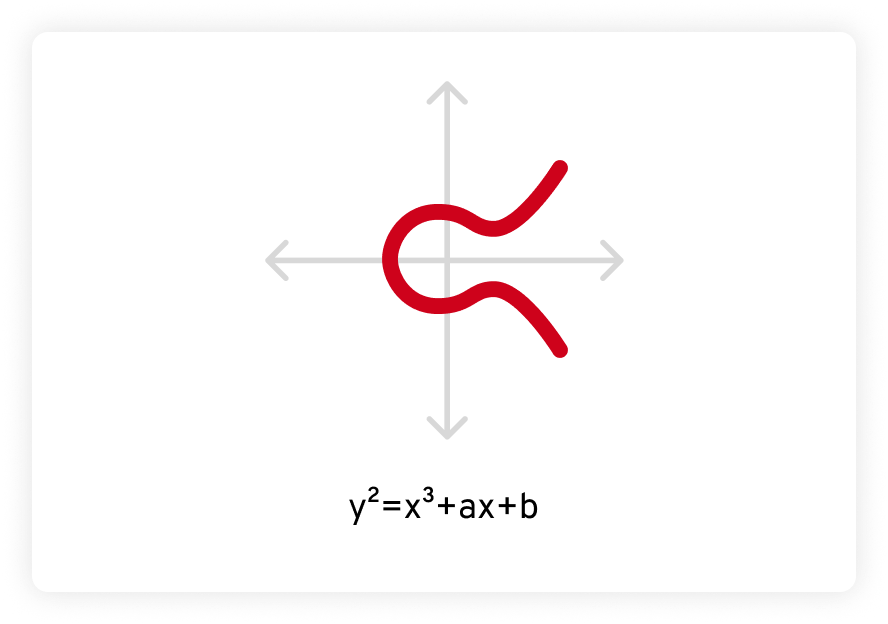
\includegraphics[width=\linewidth]{figures/image-1-1.png}
            \caption{Elliptic Curve}
            \label{fig:2}
        \end{figure}
Elliptic curves \cite{Recommendersteam} possess special mathematical properties that make them both elegant and practical for cryptographic applications. First, they exhibit horizontal symmetry, with portions on either side of the x-axis being mirror images. In addition, any line not perpendicular to the curve intersects it at no more than three points. Between points P and Q on the curve, the addition can be defined, with the sum $R = P + Q$ coordinates calculated by:
When $P \neq Q$:
$$ s = \frac{y_Q - y_P}{x_Q - x_P} $$
$$ x_R = s^2 - x_P - x_Q $$
$$ y_R = s(x_P - x_R) - y_P $$
When $P = Q$:
$$ s = \frac{3x_P^2 + a}{2y_P} $$
$$ x_R = s^2 - 2x_P $$
$$ y_R = s(x_P - x_R) - y_P $$
ECC's security is based on the difficulty of the elliptic curve discrete logarithm problem. Given a point P on the curve and a scalar k, generating a new point $Q = kP$ by multiplication of points is a forward-easy and reverse-difficult process. This one-way nature provides a solid security foundation for ECC.

\subsection{Diffie–Hellman key exchange}
In practical cryptographic systems, security alone is insufficient. In today's Internet environment, establishing shared keys through insecure channels between parties who do not know each other is a critical challenge. The Diffie-Hellman (DH) key-exchange protocol elegantly solves this problem by utilizing the discrete logarithm problem and the multiplication commutative property. In the traditional DH protocol, given a public prime p and primitive root g, both parties choose private keys a and b, then calculate and exchange public keys:
$$ A \equiv g^a \pmod{p} $$
$$ B \equiv g^b \pmod{p} $$
Finally, both parties can calculate the same shared key:
$$ S \equiv A^b \equiv B^a \equiv g^{ab} \pmod{p} $$
Protected by the discrete logarithm problem, even if an attacker knows all public information (A, B, p, g), deriving the private keys remains infeasible. This fundamental protocol enables secure communication over the Internet and forms a core component of modern encryption systems such as the Signal Protocol and TLS.
For ECC, its excellent mathematical properties allow it to replace the discrete logarithm problem in traditional DH protocols. In elliptic curves, point multiplication satisfies the commutative property:
$$ S = a(bP) = b(aP) = abP $$
This property enables ECC to serve in Diffie-Hellman key exchange, providing enhanced security and efficiency. By selecting a base point P, the parties can calculate and exchange points $A = aP$ and B = bP, ultimately obtaining the same shared key point S. This ECC-based key exchange protocol not only inherits the security features of traditional DH but also achieves better performance due to ECC's inherent advantages.

\section{Signal Protocol}
Based on DH and ECC, end-to-end encryption has achieved its initial implementation. Through encryption of the ECC curve and sharing public keys, the final key can be obtained. However, this approach faces several practical challenges. 

\begin{itemize}[noitemsep]
    \item \textbf{Key security}\newline As stated above, no encryption can be considered permanently secure, and elliptic curve encryption is no exception. Undeniably, through brute-force calculations or luck, private keys might be discovered. Keys cannot be used continuously for transmission; it is better to change them periodically, or even use different keys for each message. Thus, under current computational capabilities, each encryption remains unique, and even if one key is compromised, other information remains secure. 
    \item \textbf{Asynchrony}\newline key exchange requires both parties to be online simultaneously; otherwise, when one party is online but cannot obtain the other's key, message encryption becomes impossible. Therefore, asynchronous communication must be supported. 
    \item \textbf{The man-in-the-middle attack issue}\newline If during key exchange an intermediary intercepts both parties' public keys while generating and providing their own key, both parties believe that they are communicating with each other but are actually communicating with the intermediary. How to ensure that the sender is definitely the intended party is another problem requiring solution. 
\end{itemize}
Therefore, the Signal protocol solved these issues using multiple keys based on DH. Specifically, X3DH resolved asynchronous communication and verification in the middle, while the double-ratchet algorithm addressed the need for different keys for each message.

\subsection{X3DH}
X3DH essentially involves performing multiple DH calculations with local private keys and recipient public keys, combining them in a specific form to obtain new keys. This design enhances security by making key exchange dependent not just on single key pairs but incorporating multiple verification mechanisms. The mathematical representation of various keys is as follows:

\begin{figure}[H]
    \centering
    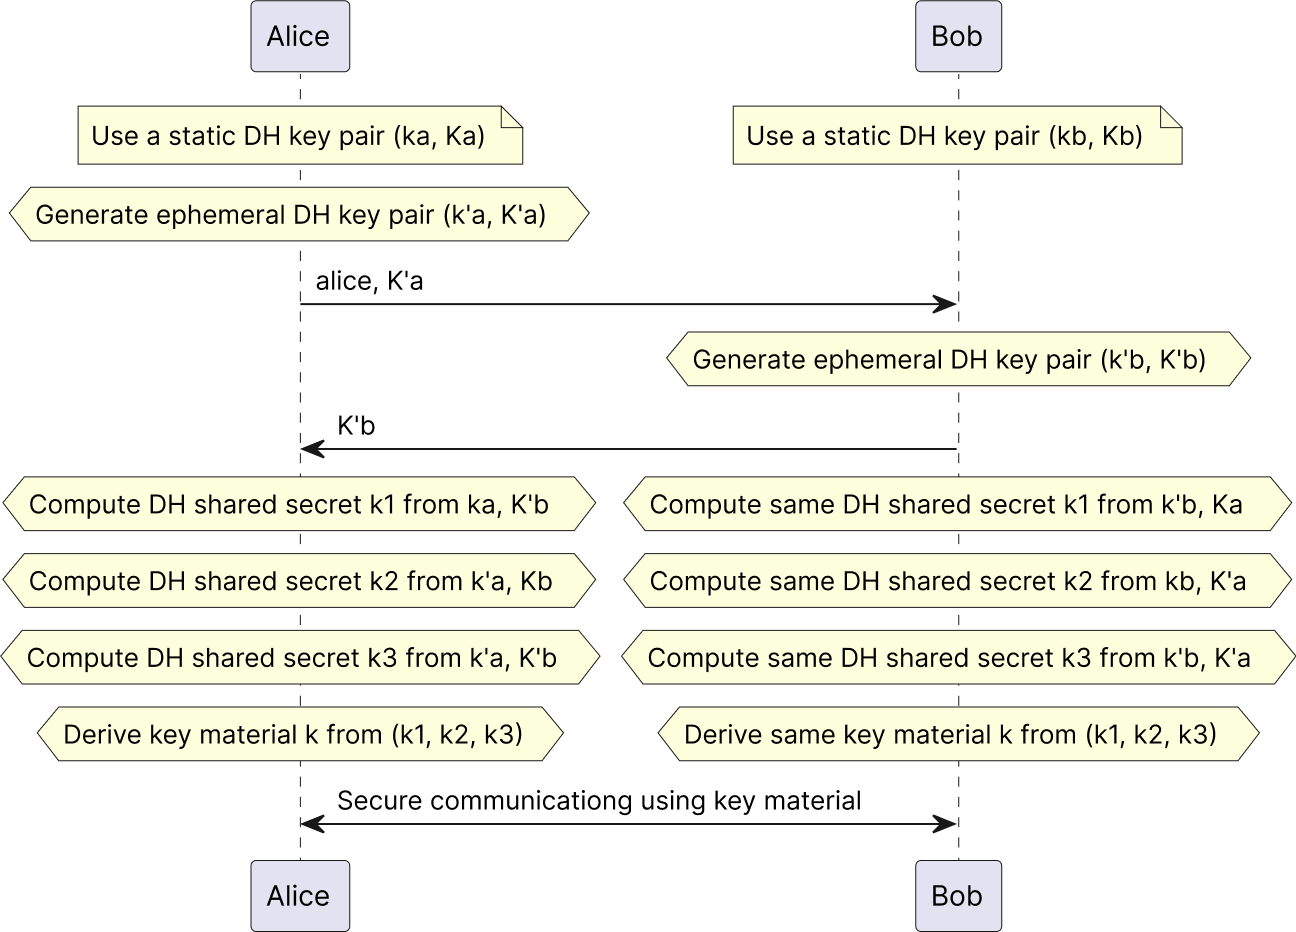
\includegraphics[width=\linewidth]{figures/image.png}
    \caption{X3DH Keypair calculate\cite{X3DH_Note}}
    \label{fig:3}
\end{figure}

\begin{itemize}
    \item \textbf{Identity Key Pair (IK)}
$$IK = (IK_{priv}, IK_{pub})$$
Long-term key pair generated when creating an account. The public key is stored on the server for mutual authentication between communicating parties, while the private key remains strictly local. As the unique identifier for each user, the IK is a permanent key that typically remains unchanged throughout the lifetime of the account unless explicitly rotated for security reasons.

\item \textbf{Signed Pre-key (SPK)}
$$SPK = (SPK_{priv}, SPK_{pub})$$
Medium-term key pair used to prevent man-in-the-middle attacks (MITM). When server support exists, each device can generate independent SPKs and update them periodically (typically every few weeks or months) to maintain security. The public key is signed by the Identity Key to prove authenticity and is published on the server, while the private key remains local.

\item \textbf{One-time Pre-key (OPK)}
$$OPK = (OPK_{priv}, OPK_{pub})$$
Single-use key pair generated in batches (typically hundreds or thousands) and stored on the server. Each OPK is used only once when establishing a new session, then permanently deleted. After use, it is removed from the server to prevent replay attacks. The client generates new OPKs as needed to maintain a sufficient pool on the server. This ensures future secrecy and uniqueness for each new conversation.

\item \textbf{Ephemeral Key (EK)}
$$EK = (EK_{priv}, EK_{pub})$$
Temporary key pair randomly generated for each new session initialization. It has the shortest lifespan of all keys - used only once for a single session setup and immediately destroyed afterward. EK enhances forward secrecy by ensuring that even if long-term keys are compromised in the future, past session keys remain secure. Each new session uses a fresh EK, guaranteeing unique shared keys for every conversation.
\end{itemize}


During key exchange, both parties perform DH calculations as follows:
Sender calculations:
$$DH_1 = IK_{A_{priv}} \cdot SPK_{B_{pub}}$$
Combines the sender's identity private key with recipient's signed pre-key. This operation verifies the recipient's identity, as only the genuine recipient possesses the corresponding SPK private key. The SPK is signed by the recipient's identity key, providing a cryptographic proof of ownership.
$$DH_2 = EK_{A_{priv}} \cdot IK_{B_{pub}}$$
Combines the sender's ephemeral private key with recipient's identity public key. This operation authenticates the sender to the recipient, as it incorporates the sender's freshly generated ephemeral key with the recipient's long-term identity key, preventing impersonation attacks.
$$DH_3 = EK_{A_{priv}} \cdot SPK_{B_{pub}}$$
$$DH_4 = EK_{A_{priv}} \cdot OPK_{B_{pub}}$$
These operations incorporate the sender's ephemeral key with the recipient's medium-term (SPK) and one-time (OPK) pre-keys. By using keys with shorter lifespans (SPK) and single-use keys (OPK), combined with the ephemeral key that's unique to each session, these operations ensure forward secrecy. Even if long-term keys are compromised in the future, past communications remain secure because these shorter-term and one-time keys are regularly rotated or used only once.

Recipient calculations:
$$DH_1 = SPK_{B_{priv}} \cdot IK_{A_{pub}}$$
$$DH_2 = IK_{B_{priv}} \cdot EK_{A_{pub}}$$
$$DH_3 = SPK_{B_{priv}} \cdot EK_{A_{pub}}$$
$$DH_4 = OPK_{B_{priv}} \cdot EK_{A_{pub}}$$
The final shared key is obtained by combining these DH values:
$$SK = KDF(DH_1 || DH_2 || DH_3 || DH_4)$$
DH operations on elliptic curves satisfy:
$$x \cdot P_{pub} = x \cdot (y \cdot G) = y \cdot (x \cdot G) = y \cdot P_{pub}$$
where G is the selected base point, x and y are private keys, and $P_{pub}$ is the corresponding public key point. Therefore, through these calculations, sender and recipient obtain identical DH values:
$$IK_{A_{priv}} \cdot SPK_{B_{pub}} = SPK_{B_{priv}} \cdot IK_{A_{pub}}$$
$$EK_{A_{priv}} \cdot IK_{B_{pub}} = IK_{B_{priv}} \cdot EK_{A_{pub}}$$
$$EK_{A_{priv}} \cdot SPK_{B_{pub}} = SPK_{B_{priv}} \cdot EK_{A_{pub}}$$
$$EK_{A_{priv}} \cdot OPK_{B_{pub}} = OPK_{B_{priv}} \cdot EK_{A_{pub}}$$
This ensures both parties can generate identical shared keys, while external attackers cannot compute the same key even if they intercept all communications. Through the use of multiple key types and multiple DH operations, the X3DH protocol achieves secure key negotiation while solving the challenges of asynchronous communication and identity authentication.

\subsection{Double Ratchet algorithm}
The Double Ratchet algorithm represents a sophisticated cryptographic protocol designed to provide robust security guarantees in asynchronous communication environments. This algorithm ensures that communicating parties can generate identical root keys during initialization, even when simultaneous communication is not possible. The protocol's primary strength lies in its ability to maintain both forward and backward secrecy of the root key and its derivatives, while ensuring unique key generation for each message exchange.

The algorithm's architecture incorporates two distinct ratchet mechanisms, hence its name: the root-key ratchet and the message ratchet. The root key ratchet facilitates the continuous evolution of the root key, while the message ratchet ensures the uniqueness of the message keys. These mechanisms are built upon the foundational Diffie-Hellman (DH) algorithm, augmented by Key Derivation Functions (KDF). The KDF serves as a critical component, transforming initial key material into purpose-specific keys, thereby enhancing the system's overall security by preventing direct usage of raw key material in data encryption operations. The KDF implementation consists of two primary phases: extraction and expansion.
The extraction phase generates a pseudorandom key (PRK) through a process involving HMAC (Hash-Based Message Authentication Code) and a salt value, expressed mathematically as
\[
\text{PRK} = \text{HMAC}_{\text{Salt}}(\text{initial\_key\_material})
\]
The subsequent expansion phase derives multiple purpose-specific keys using contextual information and counters, represented as
\[
\text{key}_1, \text{key}_2, \dots, \text{key}n = \text{HMAC}{\text{PRK}}(\text{info} || \text{counter})
\]

When a user wants to send a message, they generate an ephemeral elliptic curve (ECC) key pair. The public key from this random key pair, combined with the current root key, undergoes DH computation. The result is then passed through a KDF to derive a new root key and a message encryption key. This encryption key is used to symmetrically encrypt the message content. During transmission, the ephemeral public key is included to enable the recipient to process the message.
\begin{figure}[H]
    \centering
    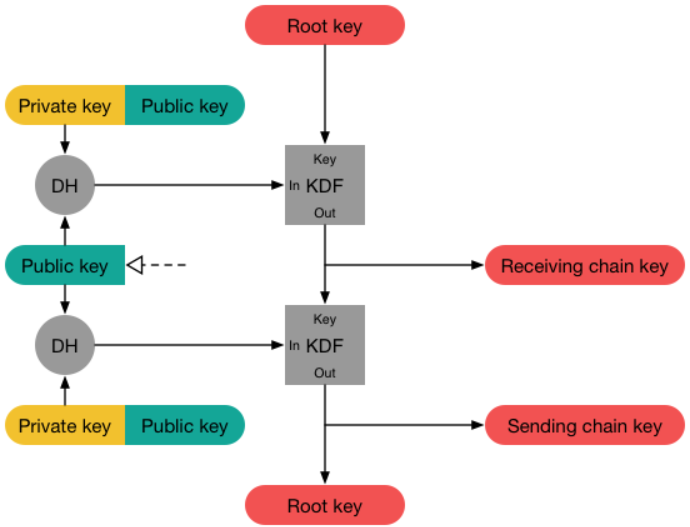
\includegraphics[width=\linewidth]{figures/Double_Ratchet_Algorithm.png}
    \caption{Double Ratchet Algorithm \cite{Double_Ratchet_Algorithm}}
    \label{fig:4}
\end{figure}

For the recipient, upon receiving the message, they extract the public key and combine it with their own root key in a DH operation. This produces a new root key and a message decryption key through the KDF. The decryption key is then used to symmetrically decrypt the message content.

The security architecture of the double-ratchet algorithm can be formally demonstrated by the following cryptographic proof. Let $(sk_r, pk_r)$ denote a randomly generated ephemeral key pair, and $mk_c$ represent the current root key. The protocol's security mechanisms operate as follows:
The sender's cryptographic operations are defined as:
$dh_r = DH(sk_r, pk_c)$ where $pk_c$ represents the current public key
\[
(mk_{\text{new}}, ck_{\text{new}}) = \text{KDF}(dh_r, \text{"root\_chain"})
\]
\[
mk = \text{KDF}(ck_{\text{new}}, \text{"message\_key"})
\]
\[ c = Enc(mk, m) \]
Similarly, the receiver's operations are:
$dh_r = DH(sk_c, pk_r)$ where $sk_c$ denotes the current private key
\[
(mk_{\text{new}}, ck_{\text{new}}) = \text{KDF}(dh_r, \text{"root\_chain"})
\]
\[
mk = \text{KDF}(ck_{\text{new}}, \text{"message\_key"})
\]
\[
m = Dec(mk, c)
\]
The security properties of the DH key exchange ensure that:
\[
DH(sk_r, pk_c) = DH(sk_c, pk_r)
\]

The deterministic nature of the KDF guarantees that when provided with identical inputs and labels ("root\_chain" and "message\_key"), both parties will derive identical $mk_{new}$, $ck_{new}$, and $mk$ values. This construction provides robust security guarantees: Even if an adversary obtains both the root key $mk_c$ and the random public key $pk_r$ at a particular point, the computational hardness of the DH problem prevents the calculation of $dh_r$. Moreover, the continuous updating of the root key with each communication ensures that compromise of a single message's encryption key does not compromise the security of other messages, effectively maintaining both forward and backward secrecy while ensuring unique key generation for each message exchange.

\section{Problem and Solution}
\subsection{ECC Vulnerabilities and Mitigation}

Curve Selection and Backdoor Risks
While Elliptic Curve Cryptography (ECC) stands as a cornerstone of modern cryptographic systems, its security fundamentally depends on the underlying curve selection. Different curves possess unique mathematical properties that directly impact both security and performance characteristics. The critical concern lies in the potential for deliberately weakened curves, where carefully chosen parameters might enable private key derivation from public keys - essentially creating a backdoor.

The Dual\_EC\_DRBG incident serves as a cautionary tale in this context. This NIST-standardized pseudorandom number generator, based on elliptic curve points, faced severe scrutiny in 2013 when evidence suggested the presence of an NSA-designed backdoor. The lack of transparency in curve parameter selection allowed potential unauthorized access to generated random numbers, highlighting the crucial importance of transparent curve design processes.

Signal Protocol's Curve Implementation
Signal Protocol addresses these concerns through its implementation of X25519 and X448, based on Curve25519 and Curve448 respectively. These curves were specifically designed with transparent generation processes, ensuring verifiable absence of backdoors. Their recognition by NIST and ANSI X9 further validates their security approach.

Key differences between these implementations:
\begin{itemize}
    \item X25519: Employs a 255-bit curve, optimized for performance, particularly suitable for resource-constrained devices and frequent key exchanges.
    \item X448: Utilizes a 448-bit prime field, offering enhanced security at the cost of computational speed, ideal for high-security applications where performance is secondary.
\end{itemize}

\subsection{Server Authentication and Security}
The Signal Protocol incorporates robust measures against man-in-the-middle attacks through two primary approaches:
\begin{itemize}
    \item SPK Signatures: Users sign their Signed Pre-Key (SPK) using their Identity Key's private component, generating SPK\_sig. This signature verifies the SPK's authenticity and origin.
    \item HTTPS Implementation: Alternatively, HTTPS protocols provide server authentication through trusted Certificate Authorities (CAs), ensuring secure key exchange and preventing tampering through TLS encryption.
\end{itemize}

\subsection{Local Security Considerations}
While Signal Protocol excels at end-to-end encryption, local device security remains crucial. Potential vulnerabilities include:

\begin{itemize}
    \item Private Key Exposure: Compromised private keys could enable message decryption and identity forgery.
    \item Session Records: Leaked session keys might compromise message confidentiality.
    \item Pre-key Vulnerabilities: Exposed pre-keys could enable future message interception.
    \item Trust Chain Compromise: Device information leaks might allow circumvention of identity verification mechanisms.
\end{itemize}

Therefore, the Signal protocol ensures that the device itself is encrypted to prevent unauthorized access. The possibility of data leaks is reduced by storing critical data encrypted in a secure hardware module.

\subsection{Quantum Computing Challenges}
The emergence of quantum computing poses a significant threat to current cryptographic systems, particularly those based on the discrete logarithm problem. While classical computers struggle with calculating x in the equation $g^x \mod p$, quantum computers using Shor's algorithm could solve this efficiently. This means that quantum computers can deduce private keys based on curves that use public keys such as ik, opk, spk, etc. in combination, so the security on which Signal's security model is based is not guaranteed.

Although large-scale quantum computers capable of breaking these systems remain years away, the cryptographic community must develop and implement quantum-resistant algorithms to ensure long-term security. The challenge lies in maintaining current security standards while preparing for the quantum computing era.

\section{Implementation}
\href{https://github.com/EnmmmmOvO/E2EE}{https://github.com/EnmmmmOvO/E2EE}

This is an end-to-end encryption program following Signal Protocol's core implementation logic. Due to time constraints and testing requirements, the Sesame protocol for multi-device management is not implemented, meaning SPK remains static without rotation, and OPK generation is limited to a one-time creation of 100 keys without replenishment. These auxiliary features are planned for future implementation.

The project is built in Rust without unsafe modules, ensuring thread safety and memory safety. It utilizes x25519-dalek's static\_secrets for generating X25519-compliant key pairs and HKDF for key derivation operations. Given the X25519 implementation, all public and private keys are 32-bit, stored in hexadecimal format both locally and on the server to minimize transmission size. A native Rust interface is created using egui for enhanced readability. Currently, private keys are stored in plaintext files for testing purposes and easy observation, though this is recognized as insecure and pending future encryption implementation.
\lstinputlisting[caption=X25519 KeyPair Generate, label={lst:listing-Mat}, language=rust]{gen.m}

During account creation, users generate IK, SPK, and OPK keys, with public keys uploaded to the server and private keys stored locally. Logging in with the same account on another device creates a new account, as message history and information cannot be accessed without explicit transfer from the old account.
\lstinputlisting[caption=Local Key Record, label={lst:listing-Mat}, language=json]{example.m}

After logging in, users can search for existing users and view both established connections and pending connection requests. For users with established connections, communication can begin immediately by utilizing the locally stored root keys.

\begin{figure}[H]
    \centering
    
\includegraphics[width=1\linewidth]{figures/Screenshot 2024-11-04 at 00.20.35.png}
    \caption{Search User}
    \label{fig:enter-label}
\end{figure}

For new connections, users can search and connect with others by obtaining their IK, SPK, and a random OPK with ID. After generating a random EK, sender-side X3DH calculation is performed, and the EK public key, OPK ID, and IK public key are sent to the server.
\lstinputlisting[caption=Sender X3DH, label={lst:listing-Mat}, language=rust]{recv.m}
\lstinputlisting[caption=Recv X3DH, label={lst:listing-Mat}, language=rust]{send.m}

When opening a chat window with a specific user, the client sends periodic requests to the server at fixed intervals to check for new incoming messages.
\begin{figure}[H]
    \centering
    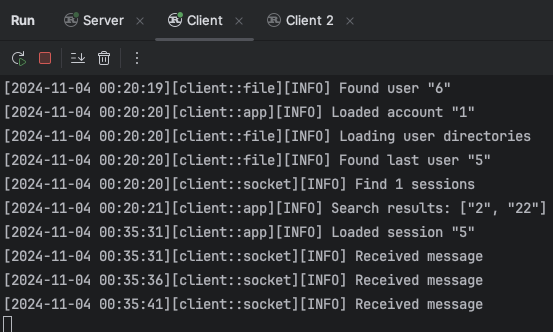
\includegraphics[width=1\linewidth]{figures/Screenshot 2024-11-04 at 00.35.45.png}
    \caption{Backend update}
    \label{fig:enter-label}
\end{figure}

When receiving a message, the system decrypts it using a combination of the local root key and the sender's random public key through the Double Ratchet Algorithm, utilizing the derived message key. 

\lstinputlisting[caption=Recv X3DH, label={lst:listing-Mat}, language=rust]{ratchet.m}

For sending messages, the system similarly employs the Double Ratchet Algorithm with the root key and a newly generated random public key, encrypting the message with the derived message key and including both the AES nonce and random public key in the transmission.

\lstinputlisting[caption=AES Encode, label={lst:listing-Mat}, language=rust]{sender.m}
\lstinputlisting[caption=AES Decode, label={lst:listing-Mat}, language=rust]{temp.m}

Message tampering tests demonstrate proper protocol behavior, with the receiving end failing to parse tampered content. 

\begin{figure}[H]
    \centering
    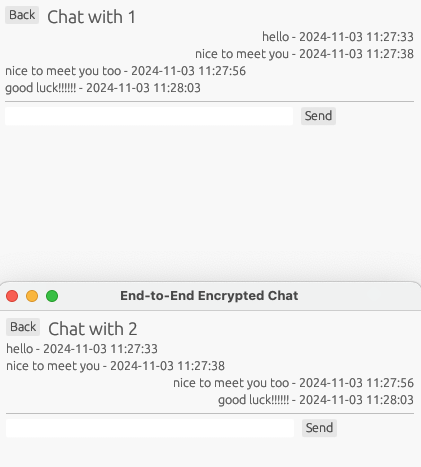
\includegraphics[width=1\linewidth]{figures/Screenshot 2024-11-03 at 22.30.24.png}
    \caption{Client}
    \label{fig:enter-label}
\end{figure}

The server uses PostgreSQL for basic storage and transmission operations, with HTTPS deployment ensuring server-side integrity in public networks.

\begin{figure}[H]
    \centering
    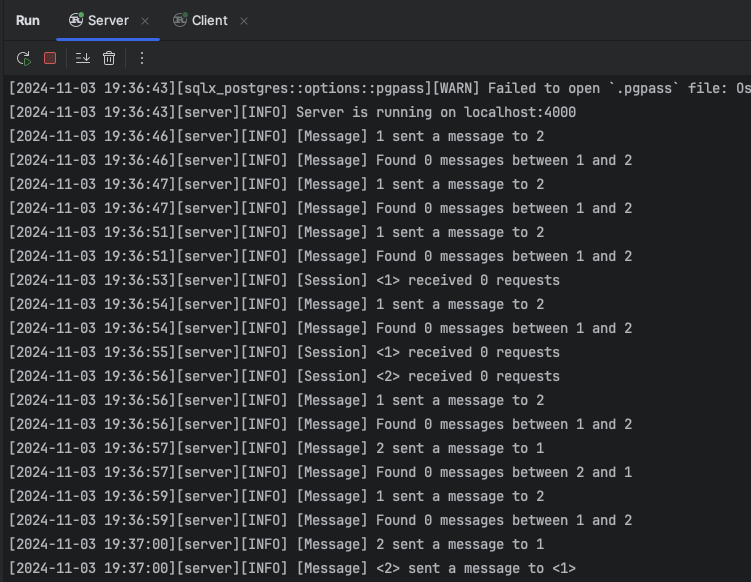
\includegraphics[width=1\linewidth]{figures/client.png}
    \caption{Server}
    \label{fig:enter-label}
\end{figure}

\section{Conclusion}
The evolution of secure communication demands robust end-to-end encryption mechanisms. Signal Protocol addresses this need through a comprehensive security approach that protects message content from the moment of creation to final delivery.

 The protocol generates unique encryption keys for each message, ensuring that even if one message is compromised, others remain secure. This security persists whether examining past or future communications.
 
The fundamental strength of Signal's end-to-end encryption lies in its layered security approach. Starting with secure key establishment through X3DH, continuing with the Double Ratchet Algorithm for ongoing message encryption, and ending with secure message delivery, each layer contributes to overall communication security. The protocol ensures that only intended recipients can access message content, while servers merely facilitate message transmission without access to content.

Security considerations span multiple dimensions. At the cryptographic level, careful curve selection prevents backdoors and ensures computational security. At the implementation level, protecting local keys and preventing man-in-the-middle attacks safeguards the encryption chain. Even as quantum computing poses future challenges to current cryptographic methods, the protocol's design principles remain valid for next-generation secure communication systems.

This examination of Signal Protocol demonstrates that effective end-to-end encryption requires both strong theoretical foundations and careful practical implementation. The protocol shows how modern cryptographic systems can provide robust security while remaining practical for everyday use.


\printbibliography

%----------------------------------------------------------

\end{document}